% ថ្នាក់ទី ១១ (វិទ្យាសាស្ត្រ) · ជំពូកទី ៨ · មេរៀនទី ២ · សៀវភៅភាគ ២ ទំព័រ ១៧០–១៧៧
\chapter{បន្ទាត់និងប្លង់ស្របក្នុងលំហ}

\begin{objBox}[វត្ថុបំណង]
\begin{enumerate}[1]
  \item កំណត់និងប្រើប្រាស់លក្ខណៈបន្ទាត់ស្របក្នុងការដោះស្រាយលំហាត់ ។
  \item កំណត់និងប្រើប្រាស់លក្ខណៈបន្ទាត់ស្របនឹងប្លង់ ក្នុងការដោះស្រាយលំហាត់ ។
\end{enumerate}
\end{objBox}

\section{បន្ទាត់ស្របគ្នា}
នៅក្នុងមេរៀនទីតាំងនៃបន្ទាត់ និងប្លង់គេបានឃើញហើយអំពីបន្ទាត់ពីរ ស្របគ្នាក្នុងប្លង់តែមួយ ។ ឧទាហរណ៍ ៖ ផ្លូវសួនច្បារចិញ្ចើមសងខាងនៃផ្លូវត្រង់មួយ $\dots$ ជារូបភាពបន្ទាត់ពីរស្របគ្នា ។

\begin{definition}[និយមន័យ]
\textbf{បន្ទាត់ពីរស្របគ្នា} គឺជាបន្ទាត់ពីរដែលនៅក្នុងប្លង់តែមួយ ហើយវាគ្មានចំណុចរួម ។
\[
d_1 \parallel d_2 \quad \text{កាលណា} \quad \begin{cases} d_1 \subset P,\ d_2 \subset P\\ d_1 \cap d_2 = \varnothing \end{cases}
\]
\end{definition}

\begin{theorem}[លក្ខណៈទី ១]
តាមចំណុចមួយស្ថិតនៅក្រៅបន្ទាត់មួយ គេអាចគូសបន្ទាត់បានតែមួយគត់ កាត់តាមចំណុចនេះ ហើយស្របទៅនឹងបន្ទាត់នោះ ។
\end{theorem}

\begin{theorem}[លក្ខណៈទី ២]
បើបន្ទាត់ពីរស្របគ្នា ហើយបន្ទាត់ទី $2$ ស្របទៅនឹងបន្ទាត់ទី $3$ នោះបន្ទាត់ទី $1$ និងទី $3$ ស្របគ្នា ៖
\[
\left.\begin{aligned} d_1 &\parallel d_2\\ d_2 &\parallel d_3 \end{aligned}\right\} \Rightarrow d_1 \parallel d_3
\]
\end{theorem}

\begin{example}[ឧទាហរណ៍ ១]
ដំបូលផ្ទះមួយ ៖ គេសង្កេតឃើញថា $d_1 \parallel d_2$ និង $d_2 \parallel d_3$ នោះ $d_1 \parallel d_3$ ។
\end{example}
\begin{example}[ឧទាហរណ៍ ២]
គេមានតុមួយ ៖ គេបាន $L_1 \parallel L_2$ និង $L_2 \parallel L_3$ នោះ $L_1 \parallel L_3$ ។
\end{example}

\begin{pro}
គេឱ្យបន្ទាត់ $a \parallel b$ ដែល $a \subset P$ និង $b \subset Q$ ហើយ $P \cap Q = l$ ។ បង្ហាញ $l \parallel a$, $l \parallel b$ ។
\ans
បើ $a$ ស្ថិតក្នុង $Q$ ផង នោះ $a = l$ ។ ករណីផ្សេង ៖ $a \parallel b$ និង $b \subset Q$ នោះ $a \parallel Q$ ។ ដោយ $a \subset P$ និង $P \cap Q = l$ នោះ $l \parallel a$ (លក្ខណៈទី ២ នៃបន្ទាត់ស្របនឹងប្លង់) ។ តាមលក្ខណៈទី ២ ខាងលើ $l \parallel a$ និង $a \parallel b$ នាំឱ្យ $l \parallel b$ ។
\end{pro}

\begin{theorem}[លក្ខណៈទី ៣]
បើបន្ទាត់ពីរស្របគ្នា គ្រប់ប្លង់ដែលកាត់បន្ទាត់ទី $1$ ត្រូវកាត់បន្ទាត់ទី $2$ ៖
\[
\left.\begin{aligned} d &\parallel d'\\ P \cap d &= \{A\} \end{aligned}\right\} \Rightarrow \text{មានចំណុច } A' \text{ ដែល } P \cap d' = \{A'\}
\]
\end{theorem}

\section{បន្ទាត់ស្របនឹងប្លង់}
បន្ទាត់ $d$ ស្របនឹងប្លង់ $P$ នោះ គេកំណត់សរសេរ $d \parallel P$ ។ ដូច្នេះ $d \parallel P \Leftrightarrow d \cap P = \varnothing$ ។
\begin{definition}[និយមន័យ]
បន្ទាត់មួយ\textbf{ស្របនឹងប្លង់}មួយ កាលណាវាគ្មានចំណុចរួម ។
\end{definition}

\begin{theorem}[លក្ខណៈទី ១]
គ្រប់បន្ទាត់ដែលនៅក្រៅប្លង់មួយ ហើយស្របនឹងបន្ទាត់មួយនៃប្លង់ជាបន្ទាត់ស្របនឹងប្លង់នោះ ៖
\[
\left.\begin{aligned} d &\not\subset P\\ d &\parallel d'\\ d' &\subset P \end{aligned}\right\} \Rightarrow d \parallel P
\]
\end{theorem}
\textbf{សម្រាយបញ្ជាក់ ៖} បន្ទាត់ស្រប $d$ និង $d'$ កំណត់បានប្លង់ $Q$ មួយដែល $P \cap Q = d'$ ។ ឧបមាថា $d \cap P = \{A\}$ មានន័យថា $A \in P$, $A \in Q$ នោះគេបាន $A \in d'$ (ព្រោះ $P \cap Q = d'$) ។ គេបាន $d \cap d' = \{A\}$ ករណីនេះ ផ្ទុយសម្មតិកម្មដែលថា $d \parallel d'$ ។ ដូច្នេះ $d$ មិនអាចកាត់ប្លង់ $P$ បានទេ ពោលគឺ $d$ ស្របនឹងប្លង់ $P$ ។

\begin{theorem}[លក្ខណៈទី ២]
បើបន្ទាត់មួយស្របនឹងប្លង់មួយ នោះគ្រប់ប្លង់ដែលកាត់តាមបន្ទាត់នេះប្រសព្វប្លង់ទី $1$ ហើយស្របនឹងបន្ទាត់នោះ ៖
\[
\left.\begin{aligned} d &\parallel P\\ d &\subset Q\\ P \cap Q &= d' \end{aligned}\right\} \Rightarrow d \parallel d'
\]
\end{theorem}
\textbf{សម្រាយបញ្ជាក់ ៖} ឧបមាថា $d \cap d' = \{A\}$ គេបាន $A \in d'$ ហើយ $A \in P$ ។ ដោយ $A \in P$ និង $A \in d$ នោះគេបាន $d$ ជួប $P$ ។ ករណីនេះផ្ទុយពីសម្មតិកម្មដែលថា $d \parallel P$ ។ ដូច្នេះ $d \parallel d'$ ($d$ និង $d'$ ស្ថិតក្នុងប្លង់ $Q$ តែមួយ) ។

\begin{example}[លំហាត់គំរូ]
គេឱ្យពីរ៉ាមីត $SABCD$ ដែលមានបាត $ABCD$ ជាការេ ។ ប្លង់មួយកាត់តាមបន្ទាត់ $BC$ ហើយប្រសព្វប្លង់ $SAD$ តាម $IJ$ ។ កំណត់ប្រភេទចតុកោណ $BCJI$ ។
\ans
គេមាន
\[
\left.\begin{aligned} BC &\parallel AD\\ AD &\subset SAD\\ BC &\not\subset SAD \end{aligned}\right\} \Rightarrow BC \parallel SAD
\]
\[
\left.\begin{aligned} BC &\parallel SAD\\ SAD \cap IBCJ &= IJ \end{aligned}\right\} \Rightarrow BC \parallel IJ
\]
ដូច្នេះ $BCJI$ ជាចតុកោណព្នាយ ។
\begin{center}
\begin{tikzpicture}[scale=1.2]
\coordinate (B) at (0,0); \coordinate (C) at (2.2,-0.6); \coordinate (D) at (3.4,0.4); \coordinate (A) at (1.2,1.0); \coordinate (S) at (1.8,3.2);
\coordinate (I) at ($(S)!0.35!(A)$); \coordinate (J) at ($(S)!0.35!(D)$);
\draw[thick] (B) -- (C) -- (D) -- (S) -- cycle (S) -- (C);
\draw[dashed] (B) -- (A) -- (D) (S) -- (A);
\draw[red,dashed] (B) -- (I) -- (J); \draw[red] (J) -- (C);
\foreach \p/\a in {A/below right,B/left,C/below,D/right,S/above,I/left,J/right} \node[\a] at (\p) {$\p$};
\end{tikzpicture}
\end{center}
\end{example}

\begin{theorem}[លក្ខណៈទី ៣]
បើបន្ទាត់មួយស្របនឹងប្លង់ពីរប្រសព្វគ្នា នោះវាស្របទៅនឹងបន្ទាត់ប្រសព្វរវាងប្លង់ទាំងពីរនោះ ៖
\[
\left.\begin{aligned} d &\parallel P\\ d &\parallel Q\\ P \cap Q &= d' \end{aligned}\right\} \Rightarrow d \parallel d'
\]
\end{theorem}
\textbf{សម្រាយបញ្ជាក់ ៖} យក $O \in d'$ ។ តាម $O$ គូសបន្ទាត់ $d'' \parallel d$ ។ គេបាន $O \in P$ នាំឱ្យ $d'' \subset P$ និង $O \in Q$ នាំឱ្យ $d'' \subset Q$ ។ នាំឱ្យ $P \cap Q = d''$ នាំឱ្យ $d''$ ត្រួត $d'$ ។ ដូច្នេះ $d \parallel d'$ ។

\section{ប្លង់ស្របគ្នា}
នៅសងខាងផ្លូវត្រង់មួយមានរបង យើងឃើញថារបងទាំងពីរនេះមិនជួបគ្នាទេ បើសិនជានៅតែមានផ្លូវបន្តទៀត ។ ដូច្នេះគេនិយាយថា ប្លង់របងទាំងពីរជាប្លង់ស្របគ្នា ។
\begin{definition}[និយមន័យ]
\textbf{ប្លង់ពីរស្របគ្នា} កាលណាវាគ្មានចំណុចរួម ។
\end{definition}
បើប្លង់ $P$ ស្របនឹងប្លង់ $Q$ នោះគេកំណត់សរសេរ $P \parallel Q$ ។ ដូច្នេះ $P \parallel Q \Leftrightarrow P \cap Q = \varnothing$ ។ (ប្លង់ឈរស្របគ្នា ប្លង់ដេកស្របគ្នា និងប្លង់ទ្រេតស្របគ្នា)
\begin{center}
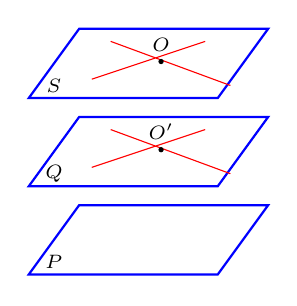
\begin{tikzpicture}[scale=0.8]
\draw[thick,blue] (0,0) -- (3,0) -- (3.8,1.1) -- (0.8,1.1) -- cycle; \node at (0.4,0.2) {\scriptsize $P$};
\draw[thick,blue] (0,1.4) -- (3,1.4) -- (3.8,2.5) -- (0.8,2.5) -- cycle; \node at (0.4,1.6) {\scriptsize $Q$};
\draw[thick,blue] (0,2.8) -- (3,2.8) -- (3.8,3.9) -- (0.8,3.9) -- cycle; \node at (0.4,3.0) {\scriptsize $S$};
\draw[red] (1.0,3.1) -- (2.8,3.7) (1.3,3.7) -- (3.2,3.0); \fill (2.1,3.38) circle (1.2pt) node[above] {\scriptsize $O$};
\draw[red] (1.0,1.7) -- (2.8,2.3) (1.3,2.3) -- (3.2,1.6); \fill (2.1,1.98) circle (1.2pt) node[above] {\scriptsize $O'$};
\end{tikzpicture}
\end{center}

\begin{theorem}[លក្ខណៈទី ១]
តាមចំណុចមួយនៅក្រៅប្លង់ $P$ មួយ គេអាចគូសបានប្លង់ $Q$ តែមួយគត់ដែលស្របទៅនឹងប្លង់នោះ ។
\end{theorem}
\begin{theorem}[លក្ខណៈទី ២]
បើប្លង់ពីរស្របគ្នា នោះគ្រប់ប្លង់ដែលស្របនឹងប្លង់មួយ ត្រូវស្របនឹងប្លង់មួយទៀត ៖
\[
\left.\begin{aligned} P &\parallel Q\\ S &\parallel Q \end{aligned}\right\} \Rightarrow P \parallel S
\]
\end{theorem}

\begin{example}[លំហាត់គំរូ ១]
គេឱ្យចតុមុខ $ABCD$ ។ $I, J, K$ និង $L$ ជាចំណុចកណ្ដាលរៀងគ្នានៃទ្រនុង $AB$, $BC$, $CD$ និង $DA$ ។ ស្រាយបញ្ជាក់ថា $IJKL$ ជាប្រលេឡូក្រាម ។
\ans
ក្នុងត្រីកោណ $ABC$ មាន $IJ$ ជាបាតមធ្យម គេបាន $IJ \parallel AC$ ។ ក្នុងត្រីកោណ $ACD$ មាន $KL$ ជាបាតមធ្យម គេបាន $KL \parallel AC$ ។ តាមលក្ខណៈទី $2$ នៃបន្ទាត់ស្របគ្នា គេបាន ៖
\[
\left.\begin{aligned} IJ &\parallel AC\\ KL &\parallel AC \end{aligned}\right\} \Rightarrow IJ \parallel KL
\]
ដូចគ្នាដែរចំពោះត្រីកោណ $ABD$ និង $BCD$ គេបាន $IL \parallel JK$ ។ ដូច្នេះ ចតុកោណ $IJKL$ មានជ្រុងពីរស្របរៀងគ្នាជាប្រលេឡូក្រាម ។
\begin{center}
\begin{tikzpicture}[scale=1.2]
\coordinate (B) at (0,0); \coordinate (C) at (2,-0.8); \coordinate (D) at (3.2,0.5); \coordinate (A) at (1.4,2.8);
\coordinate (I) at ($(A)!0.5!(B)$); \coordinate (J) at ($(B)!0.5!(C)$); \coordinate (K) at ($(C)!0.5!(D)$); \coordinate (L) at ($(D)!0.5!(A)$);
\draw[thick] (A) -- (B) -- (C) -- (D) -- cycle (A) -- (C);
\draw[dashed] (B) -- (D);
\draw[red] (I) -- (J) -- (K) -- (L) -- cycle;
\foreach \p/\a in {A/above,B/left,C/below,D/right,I/left,J/below,K/right,L/above right} \node[\a] at (\p) {$\p$};
\end{tikzpicture}
\end{center}
\end{example}

\begin{theorem}[លក្ខណៈទី ៣]
ប្លង់ពីរស្របគ្នា ហើយកាត់ដោយប្លង់ទី $3$ នោះបន្ទាត់ប្រសព្វជាបន្ទាត់ស្របគ្នា ។ គេបាន
\[
\left.\begin{aligned} P &\parallel Q\\ R \cap P &= d_1\\ R \cap Q &= d_2 \end{aligned}\right\} \Rightarrow d_1 \parallel d_2
\]
\end{theorem}
\textbf{សម្រាយបញ្ជាក់ ៖} ឧបមាថា $d_1$ ជួប $d_2$ ត្រង់ $A$ ។ គេបាន $A \in d_1 \subset P$ នោះ $A \in P$ ។ ម្យ៉ាងទៀត $A \in d_2 \subset Q$ នោះ $A \in Q$ ។ ដូច្នេះ គេបាន $A$ ជាចំណុចរួមនៃ $P$ និង $Q$ ពោលគឺផ្ទុយពីសម្មតិកម្មដែលថា $P \parallel Q$ ។ ដូច្នេះ គេបាន $d_1 \parallel d_2$ (ព្រោះ $d_1, d_2$ នៅក្នុងប្លង់ $R$ តែមួយ) ។

\begin{example}[លំហាត់គំរូ ២]
ប្លង់ $P$ និង $Q$ ជាប្លង់ស្របគ្នា ហើយ $d_1$ និង $d_2$ ជាបន្ទាត់ស្របគ្នា ។ ប្លង់ $P$ កាត់ $d_1$ និង $d_2$ រៀងគ្នាតាម $A$ និង $B$ ។ ប្លង់ $Q$ កាត់ $d_1$ និង $d_2$ រៀងគ្នាតាម $C$ និង $D$ ។ ស្រាយបញ្ជាក់ថាចតុកោណ $ABDC$ ជាប្រលេឡូក្រាម ។
\ans
ដោយបន្ទាត់ $d_1$ និង $d_2$ កំណត់ដោយប្លង់មួយដែលតាងដោយ $R$ ។ គេបានប្លង់ $R \cap P = AB$ និង $R \cap Q = CD$ ។ តាមលក្ខណៈទី $3$ គេបាន $AB \parallel CD$ ។ ម្យ៉ាងទៀត $AC \parallel BD$ (ស្ថិតលើ $d_1 \parallel d_2$) ។ ដូច្នេះ ចតុកោណ $ABDC$ ជាប្រលេឡូក្រាម ។
\end{example}

\begin{pro}
គេឱ្យប្លង់ពីរស្របគ្នា និងបន្ទាត់ពីរស្របគ្នា ដែលកាត់តាមប្លង់ពីរនោះ ។ បង្ហាញថាអង្កត់ពីរនៅចន្លោះប្លង់ពីរនោះជាអង្កត់ប៉ុនគ្នា ។
\ans
តាមលំហាត់គំរូ ២ ចតុកោណ $ABDC$ ជាប្រលេឡូក្រាម ដូច្នេះជ្រុងឈមប៉ុនគ្នា ៖ $AC = BD$ ។
\end{pro}

\begin{theorem}[លក្ខណៈទី ៤]
បើប្លង់ពីរស្របគ្នា នោះគ្រប់បន្ទាត់កាត់ប្លង់ទី $1$ ត្រូវកាត់ប្លង់ទី $2$ ៖
\[
\left.\begin{aligned} P &\parallel Q\\ d \cap P &= \{A\} \end{aligned}\right\} \Rightarrow d \cap Q = \{B\}
\]
\end{theorem}

\begin{theorem}[លក្ខណៈទី ៥]
ប្លង់ច្រើនស្របគ្នា កំណត់នៅលើខ្នាត់ពីរបានអង្កត់ត្រូវគ្នាសមាមាត្រគ្នា ។
\end{theorem}
\textbf{សម្រាយបញ្ជាក់ ៖} គេពិនិត្យប្លង់បីស្របគ្នា $P$, $Q$ និង $R$ ហើយកាត់ដោយខ្នាត់ពីរ $\Delta$ និង $\Delta'$ បានចំណុច $A, B, C$ និង $A', B', C'$ រៀងគ្នា ។ ឧបមាថាបន្ទាត់ $\Delta_1$ ស្របទៅនឹង $\Delta$ កាត់ប្លង់ $P$ ត្រង់ $A'$ ប្លង់ $Q$ ត្រង់ $B_1$ និងប្លង់ $R$ ត្រង់ $C_1$ ។ គេបាន $AB = A'B_1$, $BC = B_1C_1$ និង $AC = A'C_1$ ។ បន្ទាត់ $\Delta_1$ កាត់ $\Delta'$ ត្រង់ចំណុច $A'$ ហើយកំណត់បានប្លង់មួយ ប្លង់នេះកាត់ប្លង់ $Q$ និង $R$ តាមបន្ទាត់ $B_1B'$ និង $C_1C'$ រៀងគ្នា ដែល $B_1B' \parallel C_1C'$ ។ តាមទ្រឹស្ដីបទតាលែសគេបាន $\dfrac{A'B'}{A'B_1} = \dfrac{B'C'}{B_1C_1} = \dfrac{A'C'}{A'C_1}$ ។ ដូច្នេះគេបាន
\[
\frac{A'B'}{AB} = \frac{B'C'}{BC} = \frac{A'C'}{AC}
\]

\begin{pro}
$I, J, K$ ជាចំណុចកណ្ដាលរៀងនៃ $AE$, $BC$, $GH$ នៃគូប $ABCDEFGH$ ($ABCD$ ជាបាត ហើយ $E, F, G, H$ នៅពីលើ $A, B, C, D$ រៀងគ្នា) ។
\begin{enumerate}[a]
  \item បង្ហាញថាប្លង់ $BEG \parallel$ ប្លង់ $ACH$
  \item បង្ហាញថាប្លង់ $ICH \parallel$ ប្លង់ $KBE$
  \item បង្ហាញថាប្លង់ $IJK \parallel$ ប្លង់ $BEG$ ។
\end{enumerate}
\ans
ក. $BCHE$ និង $ABGH$ ជាចតុកោណកែង ដូច្នេះ $BE \parallel CH$ និង $BG \parallel AH$ ។ ប្លង់ $BEG$ មានបន្ទាត់ប្រសព្វពីរស្របនឹងប្លង់ $ACH$ ដូច្នេះ $BEG \parallel ACH$ ។ \quad ខ. $BE \parallel CH$ ។ តាង $M$ ជាកណ្ដាល $BE$ ៖ $IM$ និង $HK$ ស្របនិងស្មើនឹង $\tfrac{1}{2}AB$ ដូច្នេះ $HIMK$ ជាប្រលេឡូក្រាម នាំឱ្យ $HI \parallel KM$ ។ ប្លង់ $ICH$ មានបន្ទាត់ប្រសព្វ $CH$ និង $HI$ ស្របនឹងប្លង់ $KBE$ ដូច្នេះ $ICH \parallel KBE$ ។ \quad គ. តាង $N$ ជាកណ្ដាល $BG$ ៖ $\overrightarrow{IJ} = \overrightarrow{EN}$ និង $\overrightarrow{IK} = \overrightarrow{MG}$ ដូច្នេះ $IJ \parallel EN$ និង $IK \parallel MG$ ដែល $EN, MG \subset BEG$ ។ ហេតុនេះ $IJK \parallel BEG$ ។
\end{pro}

\section*{លំហាត់អនុវត្តន៍}
\begin{enumerate}[1]
  \item លំហាត់ ក. ដល់ ង. នៃគូប $ABCDEFGH$ ($ABCD$ ជាបាត, $E, F, G, H$ នៅពីលើ $A, B, C, D$ រៀងគ្នា) ចូរបញ្ជាក់ពាក្យខុសឬត្រូវ ៖ \quad ក. បន្ទាត់ $AG$ និង $DF$ ស្របគ្នា \quad ខ. បន្ទាត់ $BF$ និង $HD$ ស្របគ្នា \quad គ. ត្រីកោណ $\triangle AFH$ ជាត្រីកោណកែង \quad ឃ. បន្ទាត់ $AG$ ស្របនឹងប្លង់ $CDF$ \quad ង. ប្លង់ $ACF$ ស្របនឹងប្លង់ $EFH$ ។
  \ans
  ក. ខុស ($AG$ និង $DF$ ជាអង្កត់ទ្រូងគូប ប្រសព្វគ្នាត្រង់ផ្ចិតគូប) \quad ខ. ត្រូវ \quad គ. ខុស ($AF = FH = HA$ ជាអង្កត់ទ្រូងមុខ ៖ ត្រីកោណសមង្ស) \quad ឃ. ខុស ($AG$ កាត់ប្លង់ $CDEF$ ត្រង់ផ្ចិតគូប) \quad ង. ខុស (ប្លង់ $ACF$ កាត់ប្លង់ $EFH$ ត្រង់ $F$) ។
  \item គេឱ្យតេត្រាអែត $ABCD$ មួយ ។ បន្ទាត់ $d$ មួយកាត់តាម $A$ ស្របទៅនឹង $BC$ និង $d'$ ជាបន្ទាត់កាត់តាម $D$ ស្របទៅនឹង $AB$ ។ បង្ហាញថា $d$ និង $d'$ មិនស្ថិតក្នុងប្លង់តែមួយ ។
  \ans
  ឧបមាថា $d$ និង $d'$ ស្ថិតក្នុងប្លង់ $R$ តែមួយ ។ បើ $d \parallel d'$ នោះ $BC \parallel AB$ មិនពិត ។ ដូច្នេះ $d$ និង $d'$ ប្រសព្វគ្នា ហើយប្លង់ $R$ ស្របនឹង $BC$ និង $AB$ គឺ $R \parallel ABC$ ។ ប៉ុន្តែ $A \in R$ និង $A \in ABC$ នាំឱ្យ $R = ABC$ ដូច្នេះ $D \in ABC$ ផ្ទុយនឹង $ABCD$ ជាតេត្រាអែត ។
  \item គេមានបន្ទាត់ពីរ $a$ និង $a'$ មិនស្ថិតក្នុងប្លង់តែមួយ ។ បង្ហាញថាគ្មានបន្ទាត់ស្របគ្នាដែលកាត់តាម $a$ និង $a'$ ។
  \ans
  បើមានបន្ទាត់ $b \parallel b'$ ដែល $b$ កាត់ $a$ និង $a'$ ត្រង់ $A_1, A'_1$ ហើយ $b'$ កាត់ $a$ និង $a'$ ត្រង់ $A_2, A'_2$ នោះ $b$ និង $b'$ កំណត់ប្លង់មួយដែលមាន $A_1, A_2 \in a$ និង $A'_1, A'_2 \in a'$ ។ ដូច្នេះ $a$ និង $a'$ ស្ថិតក្នុងប្លង់នោះ ផ្ទុយនឹងសម្មតិកម្ម ។
  \item គេមានបន្ទាត់ $d$ និង $d'$ ស្របគ្នានៅក្នុងប្លង់ $P$ និង $P'$ រៀងគ្នា ។ បន្ទាត់ $a$ ជាប្រសព្វរវាងប្លង់ $P$ និង $P'$ ។ បង្ហាញថា $a \parallel d$ និង $a \parallel d'$ ។
  \ans
  $d \parallel d'$ និង $d' \subset P'$ នោះ $d \parallel P'$ (បើ $d \not\subset P'$) ។ ដោយ $d \subset P$ និង $P \cap P' = a$ តាមលក្ខណៈទី ២ នៃបន្ទាត់ស្របនឹងប្លង់ គេបាន $a \parallel d$ ។ ហើយ $a \parallel d$, $d \parallel d'$ នាំឱ្យ $a \parallel d'$ ។
  \item គេឱ្យបន្ទាត់ $a$ និង $a'$ ស្របគ្នា នៅក្នុងប្លង់ $P$ មួយ ។ ប្លង់ $Q$ និង $Q'$ កើតឡើងដោយបន្ទាត់ $a$ និង $a'$ ជាមួយនឹងបន្ទាត់ $b$ រៀងគ្នា ។ បង្ហាញថា $b$ ស្របនឹងប្លង់ $P$ ។
  \ans
  $Q \cap Q' = b$ ។ $a \parallel a' \subset Q'$ នាំឱ្យ $a \parallel Q'$ ហើយ $a \subset Q$ ដូច្នេះ $b \parallel a$ ។ ដោយ $b \parallel a \subset P$ និង $b \not\subset P$ នោះ $b \parallel P$ ។
  \item គេមានតេត្រាអែត $OABC$ មួយដែលចំណុច $M, N, P$ ជាចំណុចកណ្ដាលរៀងគ្នានៃជ្រុង $OA$, $OB$, $OC$ ។ បង្ហាញថាប្លង់ $ABC$ ស្របនឹងប្លង់ $MNP$ ។
  \ans
  $MN$ ជាបាតមធ្យមនៃ $\triangle OAB$ ៖ $MN \parallel AB$ ។ $NP$ ជាបាតមធ្យមនៃ $\triangle OBC$ ៖ $NP \parallel BC$ ។ ប្លង់ $MNP$ មានបន្ទាត់ប្រសព្វពីរ $MN$ និង $NP$ ស្របនឹងប្លង់ $ABC$ ដូច្នេះ $MNP \parallel ABC$ ។
  \item គេមានតេត្រាអែត $ABCD$ មួយដែលចំណុច $M$ ស្ថិតនៅលើជ្រុង $AB$ ខុសពី $A$ និង $B$ ។ បន្ទាត់កាត់តាមចំណុច $M$ មួយស្របទៅនឹង $AC$ រួចកាត់ $BC$ ត្រង់ $N$ ។ បន្ទាត់កាត់តាមចំណុច $N$ ស្របទៅនឹង $BD$ រួចកាត់ $CD$ ត្រង់ $P$ និងបន្ទាត់កាត់តាមចំណុច $P$ ស្របទៅនឹងបន្ទាត់ $AC$ រួចកាត់ $AD$ ត្រង់ $Q$ ។ \quad ក. បង្ហាញថា $MNPQ$ ជាប្រលេឡូក្រាម \quad ខ. បង្ហាញថា $AC$ ស្របនឹងប្លង់ $MNPQ$ ។
  \ans
  ក. $MN \parallel AC \parallel PQ$ ។ តាមទ្រឹស្ដីបទតាលែស ៖ $\dfrac{BN}{BC} = \dfrac{BM}{BA}$, $\dfrac{CP}{CD} = \dfrac{CN}{CB} = \dfrac{AM}{AB}$, $\dfrac{DQ}{DA} = \dfrac{DP}{DC} = \dfrac{BM}{AB}$ ។ ដូច្នេះ $MN = AC\cdot\dfrac{BM}{AB} = PQ$ ។ ចតុកោណ $MNPQ$ មានជ្រុងឈម $MN$ និង $PQ$ ស្របនិងប៉ុនគ្នា ជាប្រលេឡូក្រាម ។ \quad ខ. $AC \parallel MN$ និង $MN \subset MNPQ$ ហើយ $AC \not\subset MNPQ$ ដូច្នេះ $AC \parallel MNPQ$ ។
\end{enumerate}
